\documentclass[article]{article}
\usepackage[utf8]{inputenc}
\usepackage[english]{babel}
\usepackage [autostyle, english = american]{csquotes}
\MakeOuterQuote{"}

\usepackage[backend=biber,
style=authoryear,
citestyle=mla]{biblatex}
\addbibresource{refs.bib}

%% Sets page size and margins
\usepackage[letterpaper,top=3cm,bottom=2cm,left=3cm,right=3cm,marginparwidth=1.75cm]{geometry}
 
%% Useful packages
\usepackage{amsmath}
\usepackage{amssymb}
\usepackage{amsfonts}
\usepackage{mathtools}
\usepackage{graphicx}
\usepackage{enumitem}
\usepackage{hyperref}
% \usepackage{pythontex}
\usepackage{lastpage}
\usepackage{fancyhdr}
\usepackage{float}
\usepackage{csquotes}
% \usepackage{fontspec}
\usepackage{indentfirst}

\pagestyle{fancy}
\graphicspath{ {images/} }
\newcommand{\true}{$T$}
\newcommand{\false}{$F$}
\newcommand{\ans}{\textbf{Answer: }}
\newcommand{\prf}{\textbf{Proof:}}
\newenvironment{question}[2][Question]{\begin{trivlist}
\item[\hskip \labelsep {\bfseries #1}\hskip \labelsep {\bfseries #2.}]}{\end{trivlist}}

\let\emptyset\varnothing

\newenvironment{myindentpar}[1]%
  {\begin{list}{}%
          {\setlength{\leftmargin}{#1}}%
          \item[]%
  }
  {\end{list}}

\allowdisplaybreaks

\title{STAT 490, Final Project Proposal} 
\lhead{STAT 490, Final Project Proposal}

\author{Elnard Utiushev, Jessica Lynn Gilbert, Elijah Higgins}
\rhead{Elnard Utiushev, Jessica Lynn Gilbert, Elijah Higgins}
\cfoot{\thepage\ of \pageref{LastPage}}

\begin{document}

\maketitle

\tableofcontents

%% Comments
% - Paper meta analysis!!!
% - Collect case reports and do lexical analysis. Word freq.
%   - ARDS
% . - ARDS outbreak 2003
%   - MERS

% https://www.ncbi.nlm.nih.gov/pmc/articles/PMC180651/
% https://www.ncbi.nlm.nih.gov/pmc/articles/PMC3776422/


\section{Introduction}

E-cigarettes have become popular in recent years (Figure \ref{fig:vape_trend}) as what was thought to be a "safe" alternative to tobacco products. However, toward the beginning of 2019 there was a sudden increase in the number of serious injuries and deaths believed to be caused by these e-cigarettes \cite{doi:10.1056/NEJMoa1911614}.
 
The effects of vaporizer and e-cigarette use is currently a "hot topic" and a lot of conflicting information is circulating through media and research studies regarding whether they are actually safe to use. As a result, many people are unsure of whether they can trust these new tobacco alternatives.

\begin{figure}[H]
    \centering
    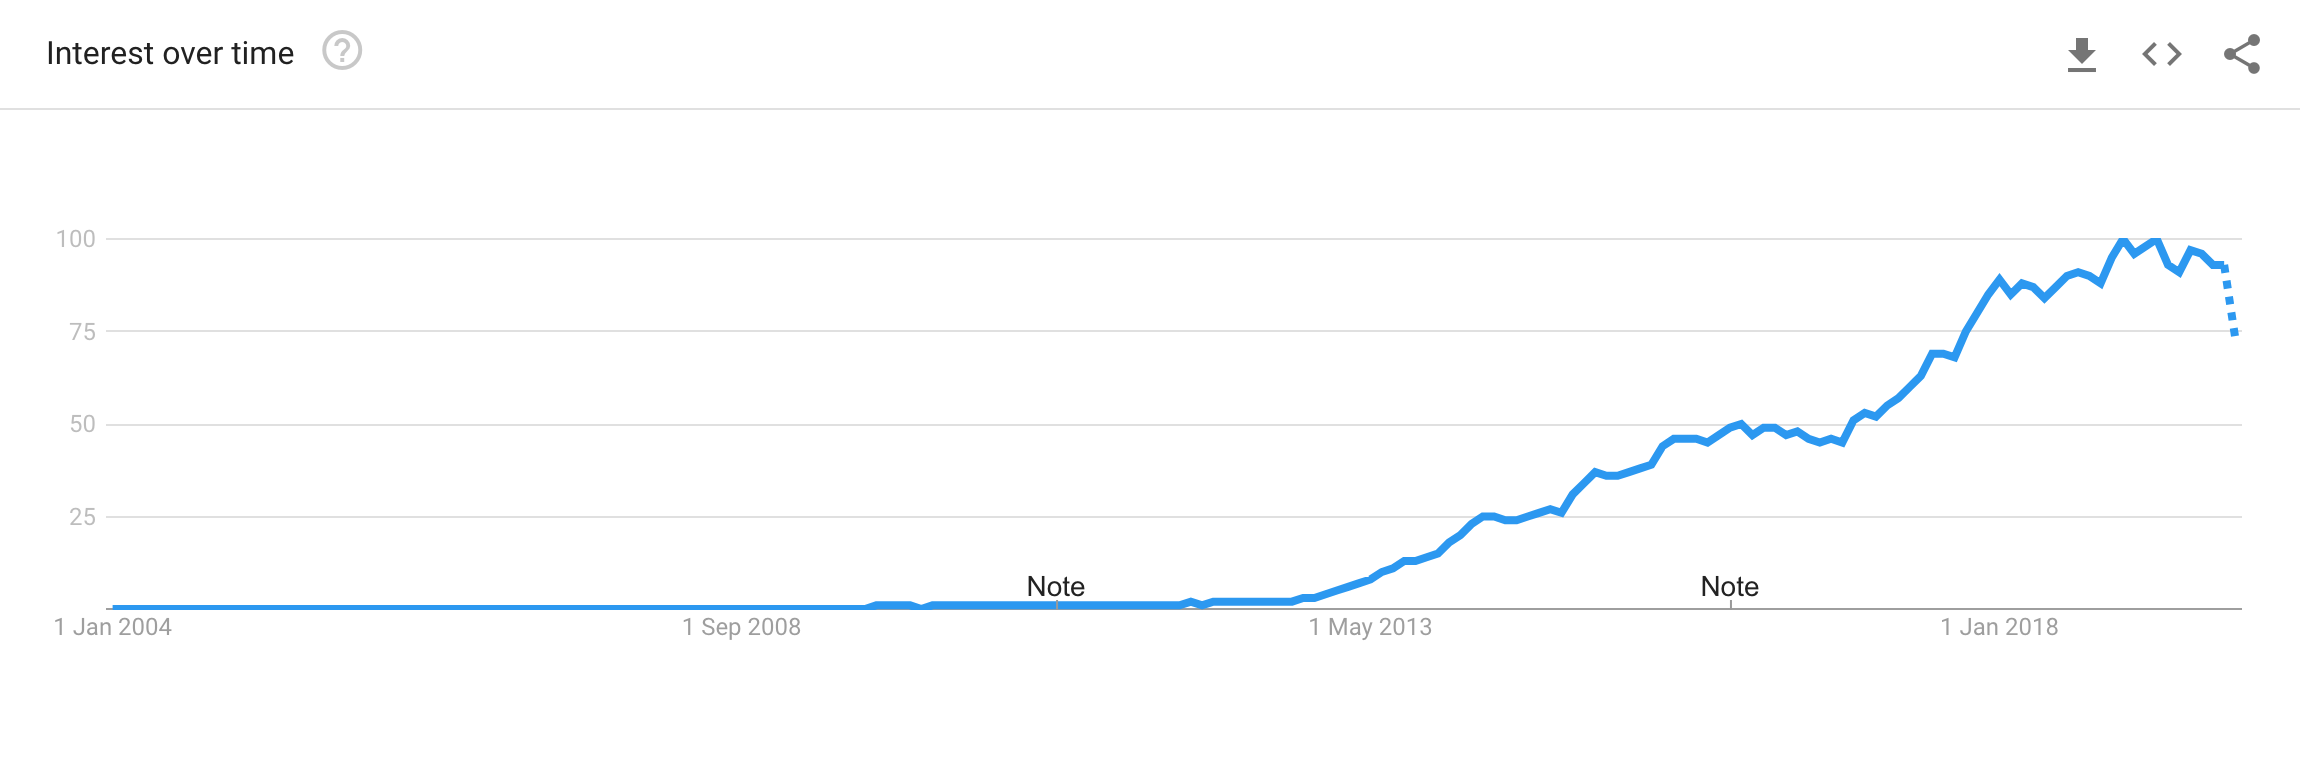
\includegraphics[width=\columnwidth]{google_trends_vape.png}
    \caption{\href{https://trends.google.com/trends/explore?date=all&geo=US&q=vape}{Google Trends Data for "vape" keyword} \cite{google_trends}}
    \label{fig:vape_trend}
\end{figure}

Thus, we propose a lexical analysis which  will compare the terminologies used in research papers and publications regarding vape-induced illnesses, acute respiratory distress syndrome (ARDs), and Middle East respiratory syndrome (MERs). We chose these two illnesses to compare with vape-induced illness and injury because they are all respiratory. Additionally, they are all serious enough that they can result in death. Through this analysis, we hope to discover the nature of the characteristics of vape-induced illnesses relative to the characteristics of ARDs and MERs. More specifically, we expect to discover any unique characteristics of vape illnesses that have not been found in cases of other respiratory illnesses, such as MERs and ARDs.

We chose a lexical analysis because any other form of study would not be possible due to ethical and logistical reasons. There is not enough data readily available for analysis nor would it be feasible to collect our own. It would be unethical to perform an experiment in which we expose subjects to vaping or other forms smoking to investigate their effects. A lexical analysis is our most coherent option. 

\section{Literature Review}
% Paper on effects of vaping: https://onlinelibrary.wiley.com/doi/full/10.1111/add.14530
% Their design was a cohort-specific simulation model of the impact of replacing smoking with nicotine vaporizing products. Their participants included two cohorts aged 30 and 50 in 2012.
% They concluded that NVP's would have a net positive impact on population health.

Middle Eastern Respiratory syndrome (MERs) is a respiratory virus which was first noted by the World Health Organization in September of 2012 for causing several cases of pneumonia, \cite{New England Journal of Medicine}. Through a case study regarding the 23 patients diagnosed with Mers-CoV, researchers concluded that the virus is capable of spreading through personal contact, especially from healthcare workers, and has a high contamination rate.

\medskip

Acute Respiratory Distress syndrome (ARDs) is a disease which gradually fills the patients lungs with fluids, depriving their organs of oxygen. However, the exact definition has changed several times since its original description in 1967, which indicates that accurately measuring incidences of this disease has been difficult. Patients usually acquire this condition through an independent injury to their lungs, or a severe injury elsewhere on their body. Therefore, some patients with ARDs do not die from the disease itself but instead from the original injury; this adds another factor to further complicate measuring of the death rates of patients with ARDs. \cite{Ware, Lorraine B and Matthay, Michael A}

\medskip

In 2019, a paper was published on the effects of smoking \cite{levy2019modeling}. Their study examined two cohorts comprised of participants aged 30 and 50 in 2012 who had known smoking patterns. The goal was to determine the impacts of replacing smoking with nicotine vaporizing products (NVP). Data on the history of smoking for each cohort to generate two simulations: one that modeled smoking rates for each cohorts life cycle in the absence of vaping and one model which considers the effects of vaping. This study found that participants in the younger cohort had fewer premature deaths and life-years lost, in the presence of NVP's.

\medskip

A publication in 2018 investigated the potential of e-cigarettes as an alternative to tobacco cigarettes. \cite{Levy18}
Their methods are described as follows:

\begin{displayquote}
A Status Quo Scenario, developed to project smoking rates and health outcomes in the absence of vaping, is compared with Substitution models, whereby cigarette use is largely replaced by vaping over a 10-year period. We test an Optimistic and a Pessimistic Scenario, differing in terms of the relative harms of e-cigarettes compared with cigarettes and the impact on overall initiation, cessation and switching. Projected mortality outcomes by age and sex under the Status Quo and E-Cigarette Substitution Scenarios are compared from 2016 to 2100 to determine public health impacts.
\end{displayquote}

\noindent
At the end of their study, researchers concluded that the replacement of tobacco cigarettes with e-cigarettes is projected to lower overall harm to smokers based on the results of both scenarios. Such a belief likely influenced recent trends in e-cigarette use.

\medskip

There is also a new paper \cite{doi:10.1056/NEJMoa1911614} which explored recent deaths caused by pulmonary illnesses in people who used vapes. They performed a case study with 53 patients. All of the patients had bilateral infiltrates. This contradicts what was previously believed about the health effects of vapes and its potential to replace tobacco cigarettes. Such contradictions surrounding e-cigarette devices are creating confusion for the public; we hope to resolve this through our analyses.

\medskip

\section{Research Design and Methods}


\begin{enumerate}
    \item Gather approximately 10 research publications regarding case studies of each type of illness (MERs, ARDs, and vape) for a total of 30 papers.
    \item Program Design
    \begin{enumerate}
        \item Extract text from the PDFs
        \item Tokenize the text with NLTK \cite{BirdKleinLoper09}
        \item Apply TF-IDF to order words according to their frequency while filtering out general words like "a" and "the".
        \item Calculate the word frequencies
    \end{enumerate}
    \item Visualize data with bar charts and Venn diagrams.
    \item Perform chi-squared tests to compare the frequencies of terms for each disease.
    \item Draw conclusions based on analyses.
\end{enumerate}

\section{Results}
Due to an unexpected lack of case study publications regarding the three illnesses, we gathered nine (9) publications regarding MERs, five (5) for ARDs, and four (4) for vape illness. After filtering out some unimportant words, plots of the most frequently-used terms still did not tell an interesting story (Figure 2). 

Next, it was decided to manually remove additional words that did not contribute to the story of our data, such as "case" and "hospital." The full list can be found in table S1. This resulted in some improvement, but not to a satisfactory level (Figure 3).

\medskip

[[[[[[[[[[[[[[[[[[[[[[[[FIGURE 2]]]]]]]]]]]]]]]]]]]]]]]]] [[[[[[[[[[[[[[[[[[[[[[[[FIGURE 3]]]]]]]]]]]]]]]]]]]]]]]]

\medskip

\noindent
A different approach was deemed necessary. Rather than manually selecting terms which we didn't want to include, we instead selected terms of interest by looking through the 200 most-frequent terms for each topic (ARDs, MERs, and vape illness). In total, 62 terms were chosen to analyze.
\medskip
(not finished, don't worry)

\clearpage

\addcontentsline{toc}{section}{References}
\printbibliography

\end{document}


